\documentclass[conference]{IEEEtran}
\IEEEoverridecommandlockouts
\usepackage[T1]{fontenc}
\usepackage{cite}
\usepackage{amsmath,amssymb,amsfonts}
\usepackage{graphicx}
\usepackage{textcomp}
\usepackage{xcolor}
\usepackage{balance}
\usepackage{booktabs}
\usepackage{caption}
\usepackage{hyperref}
\hypersetup{hidelinks}

\pagestyle{plain}

\begin{document}

\title{Post-Quantum Cryptography for MQTT Gateways:\\An Empirical Measurement Study on Commodity Edge Hardware}

\author{\IEEEauthorblockN{Sheikh Sayed Bin Rahman, Kanita Jerin Tanha, Minsoo Kim, and Taesoo Jun}
\IEEEauthorblockA{Pervasive Intelligent Computing Laboratory, Department of IT Convergence Engineering\\
Kumoh National Institute of Technology, Gumi, South Korea\\
Email: (sksayed, kanitajerin17, kms991022, taesoo.jun)@kumoh.ac.kr}}

\maketitle

\begin{abstract}
NIST has standardized several post-quantum key-encapsulation and signature families, but IoT gateway designers lack side-by-side measurements of what each choice costs on commodity edge hardware. We benchmark ten schemes---seven post-quantum KEM/signature pairings (ML-KEM, BIKE, FrodoKEM; ML-DSA, Falcon, SLH-DSA) and three classical baselines---on a Raspberry Pi MQTT gateway using real liboqs primitives, 18,000 live messages, and 5/10/100~KB payloads. At 5~KB, ML-KEM pairings with ML-DSA or Falcon require 0.56--0.77~ms median gateway cryptographic processing, 36--54\% less than classical ECDH+ECDSA (1.21~ms), because ML-KEM decapsulation outperforms P-256 scalar multiplication on the Cortex-A72, whereas code-based and unstructured-lattice KEMs require 18--37~ms. In our stateless implementation, per-message key regeneration dominates handler latency for Falcon and SLH-DSA (up to 174~ms), showing that key caching is essential.
\end{abstract}

\begin{IEEEkeywords}
Post-Quantum Cryptography, ML-KEM, ML-DSA, Falcon, SLH-DSA, MQTT, IoT Gateway, Raspberry Pi, liboqs
\end{IEEEkeywords}

\section{Introduction}

Harvest-now-decrypt-later (HNDL) adversaries record encrypted IoT traffic today and wait for a quantum computer to break the classical key exchange~\cite{shor1994,mosca2018}. NIST has standardized ML-KEM~\cite{nist_fips203}, ML-DSA~\cite{nist_fips204}, and SLH-DSA~\cite{nist_fips205}, with Falcon and alternative KEMs (BIKE, FrodoKEM) also available. Our earlier work placed the post-quantum upgrade at the MQTT gateway and measured a single pairing (ML-KEM-768 + ML-DSA-65)~\cite{rahman2025kics}. Recent IoT studies likewise evaluate one PQC configuration inside TLS~1.3 on a Raspberry Pi~4~\cite{shahid2025pqtls} or accelerate ML-KEM in dedicated ASIC hardware~\cite{dimatteo2026kem22}; these studies do not compare multiple PQC families on the same gateway, workload, and measurement pipeline.

\textbf{Contribution.} We measure ten schemes on one Raspberry Pi gateway under an identical live MQTT workload (30 scheme--payload cells, 600 messages each) and report receive-side cryptographic latency, tail latency, serialized message size, and the hidden cost of key regeneration, yielding concrete scheme recommendations for MQTT gateways.

\section{Benchmark Setup}

Each client encrypts a padded JSON payload with AES-256-GCM under a key derived from a fresh KEM encapsulation, signs it, and publishes it to a local Mosquitto broker. The gateway subscribes, decapsulates, decrypts, and verifies; we time each receive-side step with \texttt{time.perf\_counter\_ns()} and log asynchronously to avoid perturbing measurements. Gateway/device key material is reconstructed deterministically via HKDF-SHA256 from a provisioned master secret, so no key material crosses MQTT. The gateway is a Raspberry Pi~4B (Cortex-A72, 4~GB) running Python~3.11 and \texttt{liboqs-python}~\cite{oqs2023}.

We evaluate seven post-quantum pairings: ML-KEM-512 with ML-DSA-44 or Falcon-512; ML-KEM-768 with ML-DSA-65 or SLH-DSA-SHA2-128s; BIKE-L1 with ML-DSA-44; and FrodoKEM-640-AES with ML-DSA-65 or SLH-DSA-SHA2-128s. Classical baselines are two symmetric-only schemes, AES-256-GCM and ChaCha20-Poly1305, and ECDH-P256 + ECDSA-P256. Payloads are 5,120, 10,240, and 102,400 bytes. All 18,000 messages completed successfully; all signed configurations passed signature verification.

\section{Results}

\begin{table}[!t]
\centering
\captionsetup{font=footnotesize, skip=2pt}
\caption{Gateway receive cost per message (median, ms) and serialized MQTT message size. $L$ = minimum NIST security level of the pairing; real liboqs, $N=600$ per cell. ``Crypto'' = decapsulation + decryption + verification where applicable.}
\label{tab:matrix}
\footnotesize
\setlength{\tabcolsep}{2.2pt}
\begin{tabular}{lcrrrrrr}
\toprule
 & & \multicolumn{5}{c}{\textbf{5 KB payload}} & \textbf{100 KB} \\
\cmidrule(lr){3-7}
\textbf{Scheme (KEM + Sig.)} & \textbf{L} & \textbf{Decap} & \textbf{Verify} & \textbf{Crypto} & \textbf{P95} & \textbf{Msg. (B)} & \textbf{Crypto} \\
\midrule
ChaCha20-Poly1305      & -- & --     & --    & 0.073  & 0.143  & 7,327  & 0.424 \\
AES-256-GCM            & -- & --     & --    & 0.143  & 0.337  & 7,314  & 1.861 \\
ECDH + ECDSA P-256     & -- & 0.621  & 0.453 & 1.206  & 2.911  & 7,577  & 3.725 \\
\midrule
ML-KEM-512 + ML-DSA-44 & 1  & 0.130  & 0.260 & 0.562  & 1.514  & 11,604 & 3.283 \\
ML-KEM-512 + Falcon-512& 1  & 0.129  & 0.279 & 0.572  & 1.456  & 9,253  & 3.140 \\
ML-KEM-768 + ML-DSA-65 & 3  & 0.194  & 0.433 & 0.772  & 2.125  & 13,216 & 3.497 \\
ML-KEM-768 + SLH-128s  & 1  & 0.167  & 1.363 & 1.723  & 2.317  & 19,293 & 4.458 \\
Frodo-640 + ML-DSA-65  & 1  & 17.600 & 0.345 & 18.107 & 44.248 & 24,774 & 20.398 \\
Frodo-640 + SLH-128s   & 1  & 17.859 & 1.374 & 19.410 & 43.616 & 30,851 & 21.858 \\
BIKE-L1 + ML-DSA-44    & 1  & 36.126 & 0.248 & 36.550 & 54.794 & 12,677 & 39.093 \\
\bottomrule
\end{tabular}
\vspace{-3mm}
\end{table}

\begin{figure*}[!t]
\centering
\captionsetup{font=footnotesize, skip=2pt}
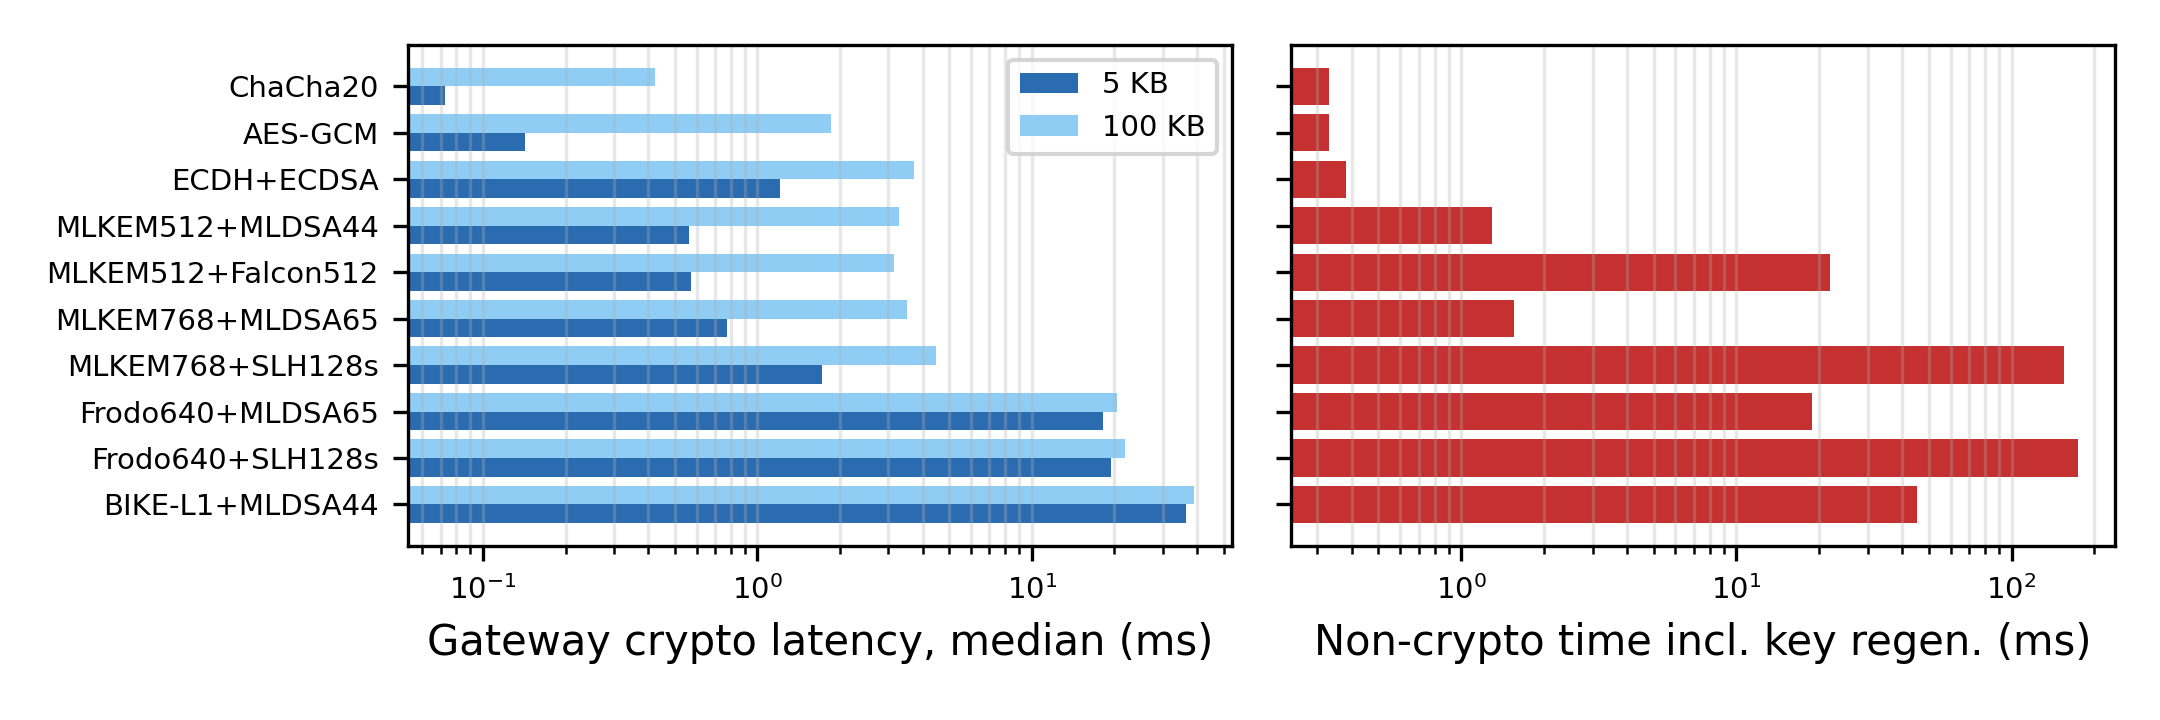
\includegraphics[width=0.9\textwidth]{figures/kics_pqc_matrix.png}
\caption{Left: gateway cryptographic latency (log scale) at 5~KB and 100~KB. Right: remaining handler time at 5~KB, dominated by per-message key regeneration for Falcon, SLH-DSA, BIKE, and FrodoKEM.}
\label{fig:matrix}
\vspace{-3mm}
\end{figure*}

\textbf{Latency.} Table~\ref{tab:matrix} and Fig.~\ref{fig:matrix} show three tiers. ML-KEM pairings with ML-DSA or Falcon require 0.56--0.77~ms gateway cryptographic processing at 5~KB, 36--54\% less than ECDH+ECDSA (1.21~ms), because ML-KEM decapsulation (0.13--0.19~ms) is 3--5$\times$ faster than P-256 ECDH scalar multiplication (0.62~ms) on the Cortex-A72. SLH-DSA verification adds about 1~ms, keeping ML-KEM-768 + SLH-DSA under 2~ms. FrodoKEM-640 (17.6~ms) and BIKE-L1 (36.1~ms) decapsulation dominate their pairings; their P95 values (44--55~ms) also show the heaviest tails. At 100~KB, AES-GCM decryption grows to about 1.9~ms and narrows the gap: ML-KEM-768 + ML-DSA-65 costs only 1.9$\times$ symmetric-only AES (3.50 vs.\ 1.86~ms). Results at 10~KB lie between the two sizes for every scheme.

\textbf{Bandwidth.} Even the AES baseline expands the 5,120-byte payload to a 7,314-byte serialized message (+43\%): Base64 encoding of the 5,136-byte ciphertext (payload + 16-byte GCM tag) yields 6,848~bytes, and JSON metadata (device, session, sequence, algorithm fields, nonce) adds about 466~bytes. At 5~KB, post-quantum material enlarges the message over the AES baseline by 1.27$\times$ (Falcon-512) to 4.22$\times$ (FrodoKEM + SLH-DSA). Because this overhead is fixed per message, it shrinks to 1.4--17\% at 100~KB, favouring batching of small sensor readings before PQC protection.

\textbf{Hidden cost of key regeneration.} In our stateless implementation, the full handler also regenerates the gateway KEM key pair and device verification key for every message. For ML-KEM/ML-DSA this adds only 1.3--1.6~ms, but Falcon-512 adds 22~ms, FrodoKEM 19~ms, BIKE 45~ms, and SLH-DSA 155--174~ms (Fig.~\ref{fig:matrix}, right), about 90$\times$ the cryptographic work itself. Practical gateways should therefore cache key pairs per device and KEM rather than rederiving them.

\textbf{Recommendation.} For MQTT gateways, ML-KEM-768 + ML-DSA-65 offers NIST Level~3 at under 0.8~ms and a 5.9~KB per-message overhead; ML-KEM-512 + Falcon-512 is the most bandwidth-efficient Level~1 option; SLH-DSA suits conservative deployments if keys are cached; FrodoKEM and BIKE are better suited to latency-tolerant links.

\section{Conclusion}

On a Raspberry Pi MQTT gateway, receive-side ML-KEM pairings with ML-DSA or Falcon are faster than classical ECDH+ECDSA, while FrodoKEM and BIKE pairings are 23--47$\times$ slower than ML-KEM-768 + ML-DSA-65 and enlarge messages substantially. Key caching, not algorithm choice alone, determines whether Falcon and SLH-DSA are practical. Future work will add energy measurements and multi-gateway deployments.

\noindent\textbf{Acknowledgment.} Funded by NRF (MSIT; RS-2026-25497739, 34\%), IITP Innovative Human Resource Development for Local Intellectualization (MSIT; IITP-2026-RS-2020-II201612, 33\%), and NRF Basic Science Research Program (MOE; 2018R1A6A1A03024003, 33\%).
\balance

\begin{thebibliography}{9}
\footnotesize

\bibitem{shor1994}
P.~W. Shor, ``Algorithms for quantum computation: Discrete logarithms and factoring,'' in \textit{Proc. 35th FOCS}, 1994, pp.~124--134.

\bibitem{mosca2018}
M.~Mosca, ``Cybersecurity in an era with quantum computers: Will we be ready?'' \textit{IEEE Secur. Privacy}, vol.~16, no.~5, pp.~38--41, 2018.

\bibitem{nist_fips203}
NIST, \textit{FIPS 203: Module-Lattice-Based Key-Encapsulation Mechanism Standard}, 2024.

\bibitem{nist_fips204}
NIST, \textit{FIPS 204: Module-Lattice-Based Digital Signature Standard}, 2024.

\bibitem{nist_fips205}
NIST, \textit{FIPS 205: Stateless Hash-Based Digital Signature Standard}, 2024.

\bibitem{rahman2025kics}
S.~S.~B. Rahman, W.~N.~B.~W.~M. Nasir, K.~J. Tanha, and T.~Jun, ``A two-stage Raspberry Pi security pipeline for military IoT attack filtering and quantum-safe cloud transit,'' in \textit{Proc. KICS Conf.}, 2025.

\bibitem{shahid2025pqtls}
A.~B. Shahid, K.~Mansoor, Y.~A. Bangash, W.~Iqbal, and S.~Mussiraliyeva, ``Post-quantum cryptographic authentication protocol for industrial IoT using lattice-based cryptography,'' \textit{Sci. Rep.}, vol.~16, Art.~9582, 2026, doi: 10.1038/s41598-025-28413-8.

\bibitem{dimatteo2026kem22}
S.~Di~Matteo, I.~Sarno, E.~Valea, and S.~Saponara, ``KEM-22: An efficient post-quantum ML-KEM hardware accelerator on 22-nm ASIC,'' \textit{IEEE Internet Things J.}, vol.~13, no.~3, pp.~4715--, Feb. 2026, doi: 10.1109/JIOT.2025.3635477.

\bibitem{oqs2023}
Open Quantum Safe Project, ``liboqs: Open-source quantum-safe cryptography library,'' 2023. [Online]. Available: \url{https://openquantumsafe.org}

\end{thebibliography}

\end{document}
